\subsection{Gini Index}
\textit{Gini index}\cite{ginindex} measures the inequality of a
distribution. Values of 0 and 1 stand for, respectively, the
maximum homogeneity and the maximum heterogeneity.
However, this index is a function of random values: mean and
error have to be estimated.\\
A certain number of samples is created by sampling with replacement
of the average FOUR distribution: Gini index is computed for each
one of them.
Now we have a population of Gini indexes, and we can extract
mean and error: the whole process is known as
\textit{bootstrap}.\footnote{See \nameref{Appendix A} for error estimation.}\cite{bootstrap}\\
In practical terms, for every level of  memory, a simulation with
twenty news is run out: Gini index' mean and error are computed
like before.
The Gini index-memory plot shows a highly non-linear behaviour:
sigmoid and gaussian seem to better represent data.\\
In order to select the best-fit function, \textit{Chi-square} is
computed for both of them. \\
Because of asymmetric error bars, the optimization function is
slightly different from the standard one, used for weighted
interpolation.\footnote{See \nameref{Appendix B} for more details.}
The overall results are shown below:
%
%\begin{figure}[!h]
  %\centering
  %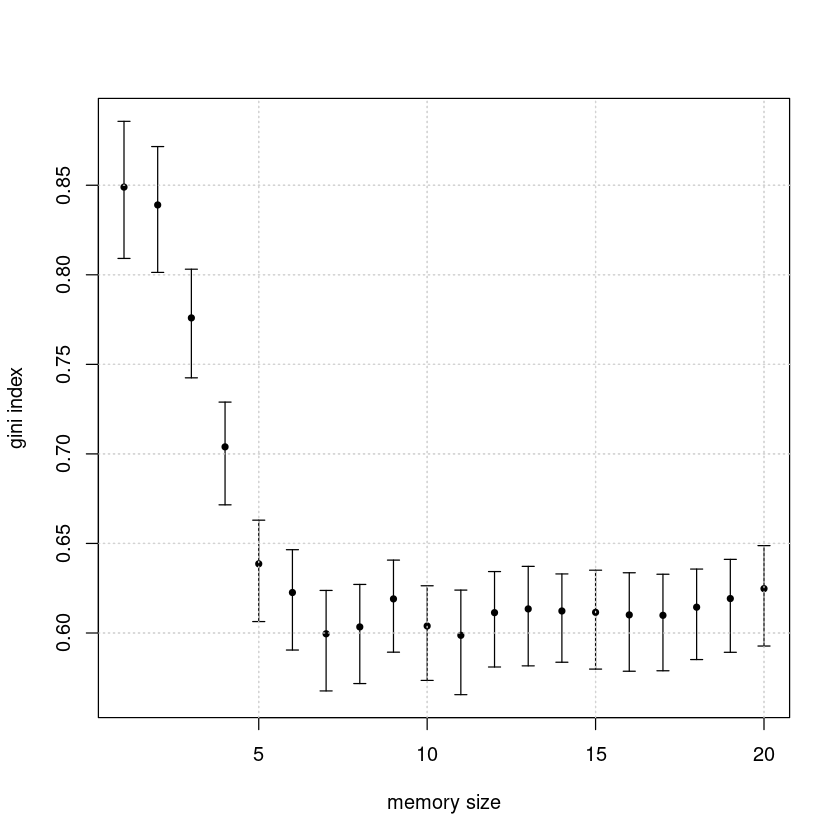
\includegraphics[width=.7\columnwidth]{img/gini_memory.png}
  %\caption{Gini index-memory plot with errorbars}
  %\label{fig:ginimem}
%\end{figure}
%
\begin{figure}[h]
  \centering
  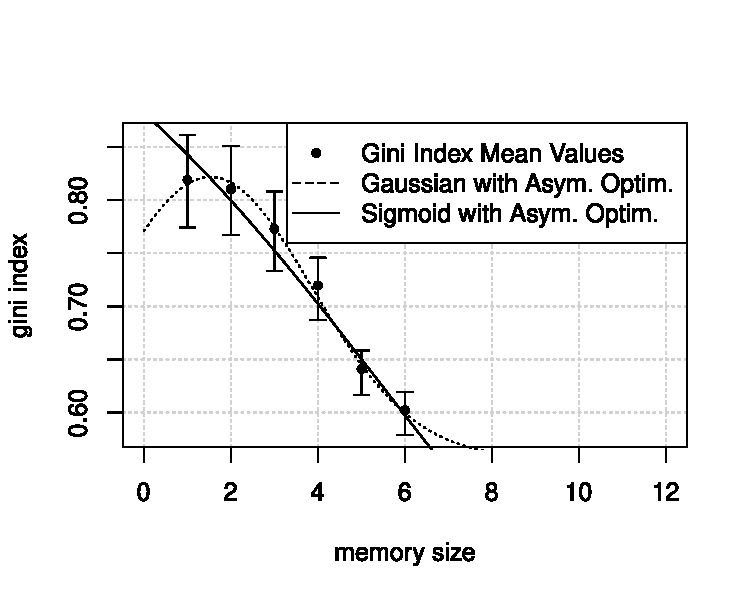
\includegraphics[trim={0cm 0cm 0cm 1cm},clip,width=.8\columnwidth]{img/gini.pdf}
  \caption[Gini index on memory size]
  {Gini index of fraction of users reached on memory size
    fitted with Gaussian and Sigmoid.
  }
  \label{fig:gini}
\end{figure}
%
\begin{table}[h]
  \centering
  \begin{tabular}{lcccc}
    \toprule
    & \multicolumn{2}{c}{\textit{Gaussian Fit}} & \multicolumn{2}{c}{\textit{Sigmoid Fit}}\\
     & {$\chi^2$} & {p-value} & {$\chi^2$} & {p-value} \\ \midrule
    \textit{std. err.} & \SI{1.3e-3}{} & \SI{9.7e-1}{} & \SI{8.1e-4}{} & \SI{9.8e-1}{} \\
    %\midrule[0.01em]
    \cmidrule(lr{0.01em}){2-5}
    \textit{quant. err.} & \SI{3.7e-3}{} & \SI{9.5e-1}{} & \SI{1.3e-3}{}  & \SI{9.7e-1}{} \\
    \textit{asym. err.} & \SI{1.4e-3}{} & \SI{9.7e-1}{} & \SI{8.4e-4}{} & \SI{9.8e-1}{} \\ \bottomrule
  \end{tabular}
  \caption[Reduced $\chi^2$ and p-value for Gaussian and Sigmoid fit]
  {Reduced $\chi^2$ and respective p-value for Gaussian
    and Sigmoid fit with different non-linear optimization
    strategies.\\
    Optimization using the standard error of the Gini index
    is denoted as std, quantile bootstrap optimization\cite{quantile} as
    quant and asymmetric error bar fitting optimization as asym.}
  \label{tab:gini}
\end{table}
%
We can notice that, for every type of errorbar, sigmoid's
$\chi^2$ is slightly lower than gaussian one; p-value is
higher instead.
Null hypothesis, for both measures, is far from being rejected:
goodness-of-fit is solidly validated.
Hence, sigmoid is our best-fit function for gini index-memory
length plot.
